% Options for packages loaded elsewhere
\PassOptionsToPackage{unicode}{hyperref}
\PassOptionsToPackage{hyphens}{url}
%
\documentclass[
  10pt,
  b5paper,
  oneside]{book}
\usepackage{amsmath,amssymb}
\usepackage{lmodern}
\usepackage{iftex}
\ifPDFTeX
  \usepackage[T1]{fontenc}
  \usepackage[utf8]{inputenc}
  \usepackage{textcomp} % provide euro and other symbols
\else % if luatex or xetex
  \usepackage{unicode-math}
  \defaultfontfeatures{Scale=MatchLowercase}
  \defaultfontfeatures[\rmfamily]{Ligatures=TeX,Scale=1}
\fi
% Use upquote if available, for straight quotes in verbatim environments
\IfFileExists{upquote.sty}{\usepackage{upquote}}{}
\IfFileExists{microtype.sty}{% use microtype if available
  \usepackage[]{microtype}
  \UseMicrotypeSet[protrusion]{basicmath} % disable protrusion for tt fonts
}{}
\makeatletter
\@ifundefined{KOMAClassName}{% if non-KOMA class
  \IfFileExists{parskip.sty}{%
    \usepackage{parskip}
  }{% else
    \setlength{\parindent}{0pt}
    \setlength{\parskip}{6pt plus 2pt minus 1pt}}
}{% if KOMA class
  \KOMAoptions{parskip=half}}
\makeatother
\usepackage{xcolor}
\usepackage{longtable,booktabs,array}
\usepackage{calc} % for calculating minipage widths
% Correct order of tables after \paragraph or \subparagraph
\usepackage{etoolbox}
\makeatletter
\patchcmd\longtable{\par}{\if@noskipsec\mbox{}\fi\par}{}{}
\makeatother
% Allow footnotes in longtable head/foot
\IfFileExists{footnotehyper.sty}{\usepackage{footnotehyper}}{\usepackage{footnote}}
\makesavenoteenv{longtable}
\usepackage{graphicx}
\makeatletter
\def\maxwidth{\ifdim\Gin@nat@width>\linewidth\linewidth\else\Gin@nat@width\fi}
\def\maxheight{\ifdim\Gin@nat@height>\textheight\textheight\else\Gin@nat@height\fi}
\makeatother
% Scale images if necessary, so that they will not overflow the page
% margins by default, and it is still possible to overwrite the defaults
% using explicit options in \includegraphics[width, height, ...]{}
\setkeys{Gin}{width=\maxwidth,height=\maxheight,keepaspectratio}
% Set default figure placement to htbp
\makeatletter
\def\fps@figure{htbp}
\makeatother
\setlength{\emergencystretch}{3em} % prevent overfull lines
\providecommand{\tightlist}{%
  \setlength{\itemsep}{0pt}\setlength{\parskip}{0pt}}
\setcounter{secnumdepth}{5}
\usepackage{booktabs}
\usepackage{amsthm}
\makeatletter
\let\stdl@chapter\l@chapter
\renewcommand*{\l@chapter}[2]{%
  \stdl@chapter{\textcolor{astral}{#1}}{\textcolor{astral}{#2}}}

\def\thm@space@setup{%
  \thm@preskip=5cm
  \thm@postskip=\thm@preskip

}
\usepackage{graphicx}
\usepackage{afterpage}

\newcommand\blankpage{%
    \null
    \thispagestyle{empty}%
    \addtocounter{page}{-1}%
    \newpage}

\usepackage{amssymb}
\usepackage{amsmath}
%\pagestyle{plain} % default for report

\usepackage{etoolbox}
\makeatletter
\patchcmd{\@makechapterhead}{50\p@}{-24pt}{}{}
\patchcmd{\@makeschapterhead}{50\p@}{-24pt}{}{}
\makeatother

\makeatother
\usepackage{sectsty}

\definecolor{astral}{RGB}{153, 61, 15}
\allsectionsfont{\sffamily\color{astral}}


\usepackage{fancyhdr}
\usepackage{pdfpages}

\renewcommand{\headrulewidth}{0.5pt}
\renewcommand{\headrule}{\hbox to\headwidth{\color{astral}\leaders\hrule height \headrulewidth\hfill}}


\setlength{\headheight}{5pt}

\fancyhf{}
\fancyhead[EL]{\nouppercase\leftmark}
\fancyhead[OR]{\nouppercase\rightmark}
\fancyhead[ER,OL]{\thepage}

\usepackage{multicol}
\usepackage{hyperref}
\usepackage{longtable}
\usepackage{array}
\usepackage{multirow}
\usepackage{wrapfig}
\usepackage{float}
\usepackage{colortbl}
\usepackage{pdflscape}
\usepackage{tabu}
\usepackage{threeparttable}
\usepackage{adjustbox}
\usepackage{rotating}
\usepackage{tablefootnote}
\usepackage[normalem]{ulem}
% empty pages betwen chapters
\usepackage{emptypage}


\makeatletter
\makeatother

\renewcommand{\listfigurename}{Figures}
\renewcommand{\listtablename}{Tables}

\usepackage[sectionbib]{chapterbib}

%% List of Abbreviations
\usepackage{nomencl}
\makenomenclature
\renewcommand{\nomname}{Acronyms}
%% to update run makeindex on docs folder and move results to / folder
%% see nomencl manual
%% e.g. makeindex SOCMapping.nlo -s nomencl.ist -o SOCMapping.nls

%% index
\usepackage{imakeidx}
\makeindex

\usepackage{xspace}

% no title page
\AtBeginDocument{\let\maketitle\relax}
\hypersetup{
	colorlinks=true,
	linkcolor=astral,
	filecolor=astral,
	urlcolor=astral,
	citecolor=astral
}
\AtBeginDocument{\renewcommand{\chaptername}{Chapter}}
\usepackage{titling}
\usepackage{natbib}
\usepackage{pdfpages}
\usepackage{fancyhdr}
\usepackage{booktabs}
\usepackage{longtable}
\usepackage{subfig}
\usepackage{array}
\usepackage{amsmath}
\usepackage{multirow}
\usepackage{wrapfig}
\usepackage{bookmark}
\usepackage[utf8]{inputenc}
\usepackage{float}
\usepackage{colortbl}
\usepackage{pdflscape}
\usepackage{tabu}
\usepackage{threeparttable}
\usepackage{threeparttablex}
\usepackage[normalem]{ulem}
\usepackage{makecell}
\usepackage{xcolor}
\DeclareUnicodeCharacter{2212}{\textendash}
\usepackage{rotating, graphicx}
\usepackage{booktabs}
\usepackage{longtable}
\usepackage{array}
\usepackage{multirow}
\usepackage{wrapfig}
\usepackage{float}
\usepackage{colortbl}
\usepackage{pdflscape}
\usepackage{tabu}
\usepackage{threeparttable}
\usepackage{threeparttablex}
\usepackage[normalem]{ulem}
\usepackage{makecell}
\usepackage{xcolor}
\ifLuaTeX
  \usepackage{selnolig}  % disable illegal ligatures
\fi
\IfFileExists{bookmark.sty}{\usepackage{bookmark}}{\usepackage{hyperref}}
\IfFileExists{xurl.sty}{\usepackage{xurl}}{} % add URL line breaks if available
\urlstyle{same} % disable monospaced font for URLs
\hypersetup{
  pdftitle={ Technical Manual for Global Soil Nutrient and Nutrient Budgets map (GSNmap)},
  pdfauthor={Angelini, M.E, Mainka, M., Luotto, I., Omuto Thine, C., Yigini, Y., Tong, Y.},
  hidelinks,
  pdfcreator={LaTeX via pandoc}}

\title{
Technical Manual for Global Soil Nutrient and Nutrient Budgets map (GSNmap)}
\usepackage{etoolbox}
\makeatletter
\providecommand{\subtitle}[1]{% add subtitle to \maketitle
  \apptocmd{\@title}{\par {\large #1 \par}}{}{}
}
\makeatother
\subtitle{version 0.2}
\author{Angelini, M.E, Mainka, M., Luotto, I., Omuto Thine, C., Yigini, Y., Tong, Y.}
\date{26-Oct-2022}

\begin{document}
\maketitle

\pagestyle{plain}
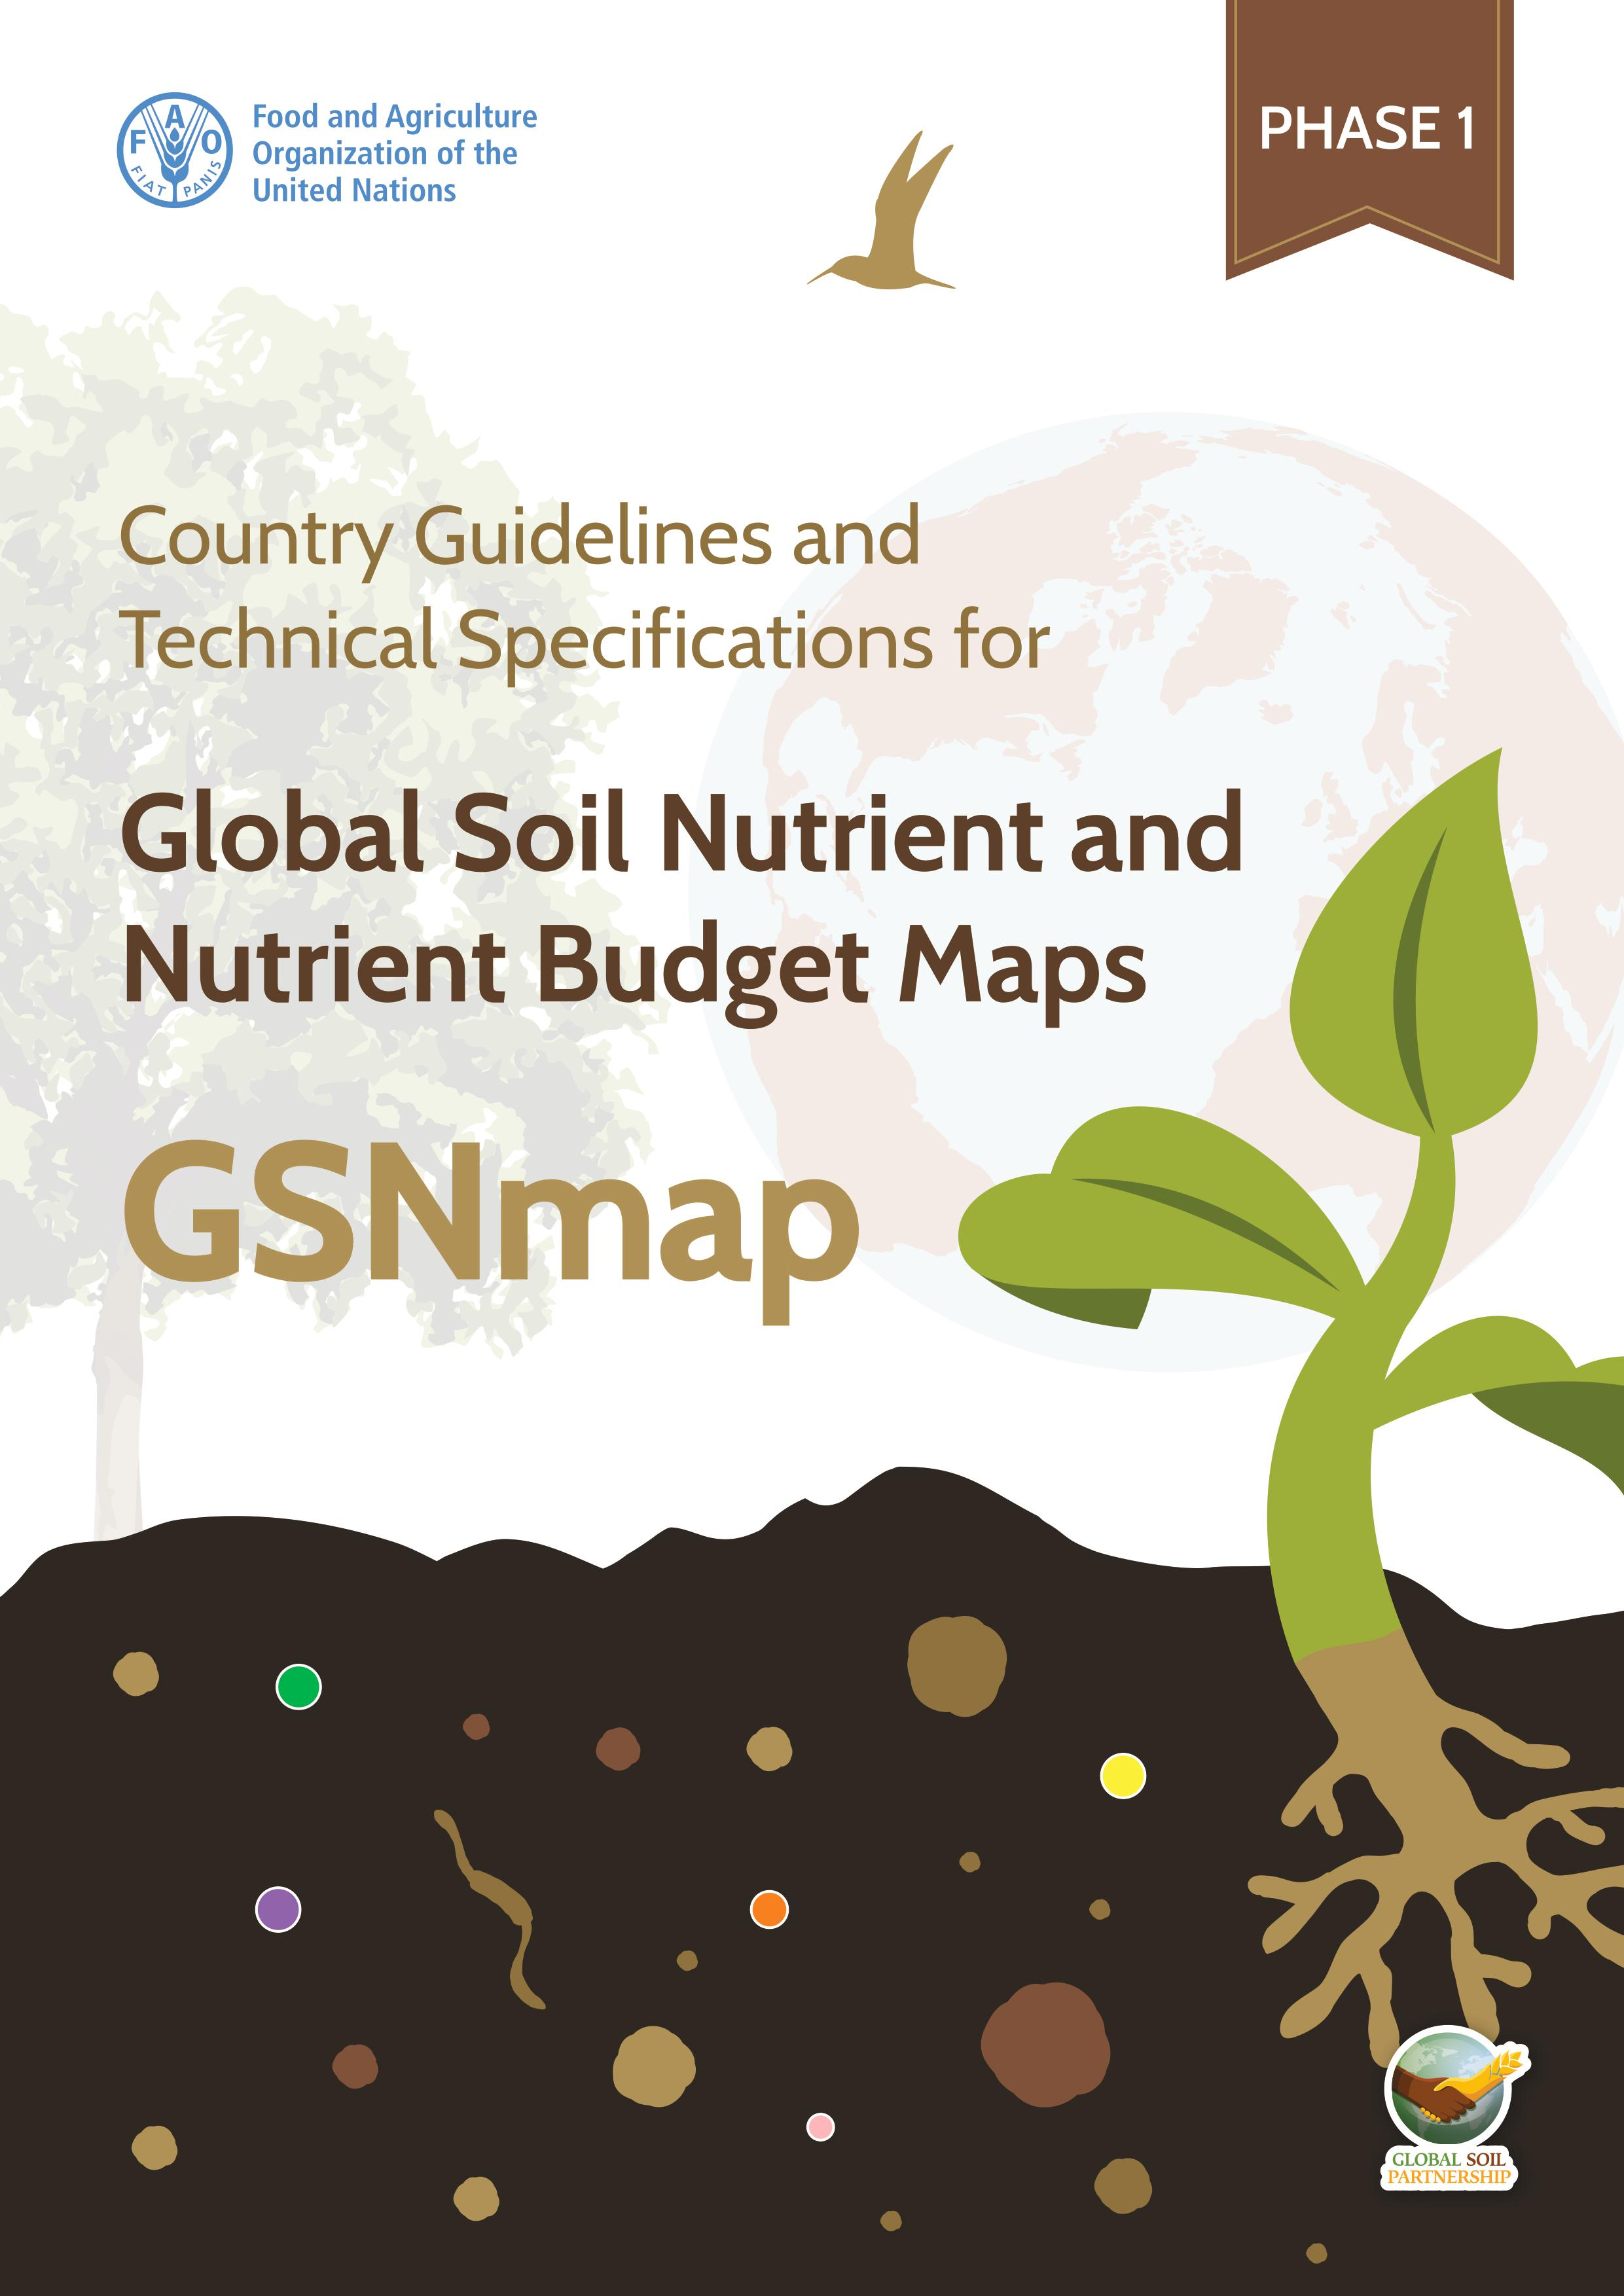
\includepdf{images/frontcover.pdf}
\afterpage{\blankpage}
\thispagestyle{empty}
\begin{titlepage}
    \begin{center}
        \vspace*{4cm}
        \Large

        \textcolor{astral}{\textbf{Country Guidelines on Digital Soil Mapping\\}}
        \vspace{0.5cm}
        \normalsize
        \vfill
        \noindent
        {\color{astral}\rule{\linewidth}{0.5mm} }

        Food and Agriculture Organization of the United Nations\\
	Rome, 2022
    \end{center}
\end{titlepage}
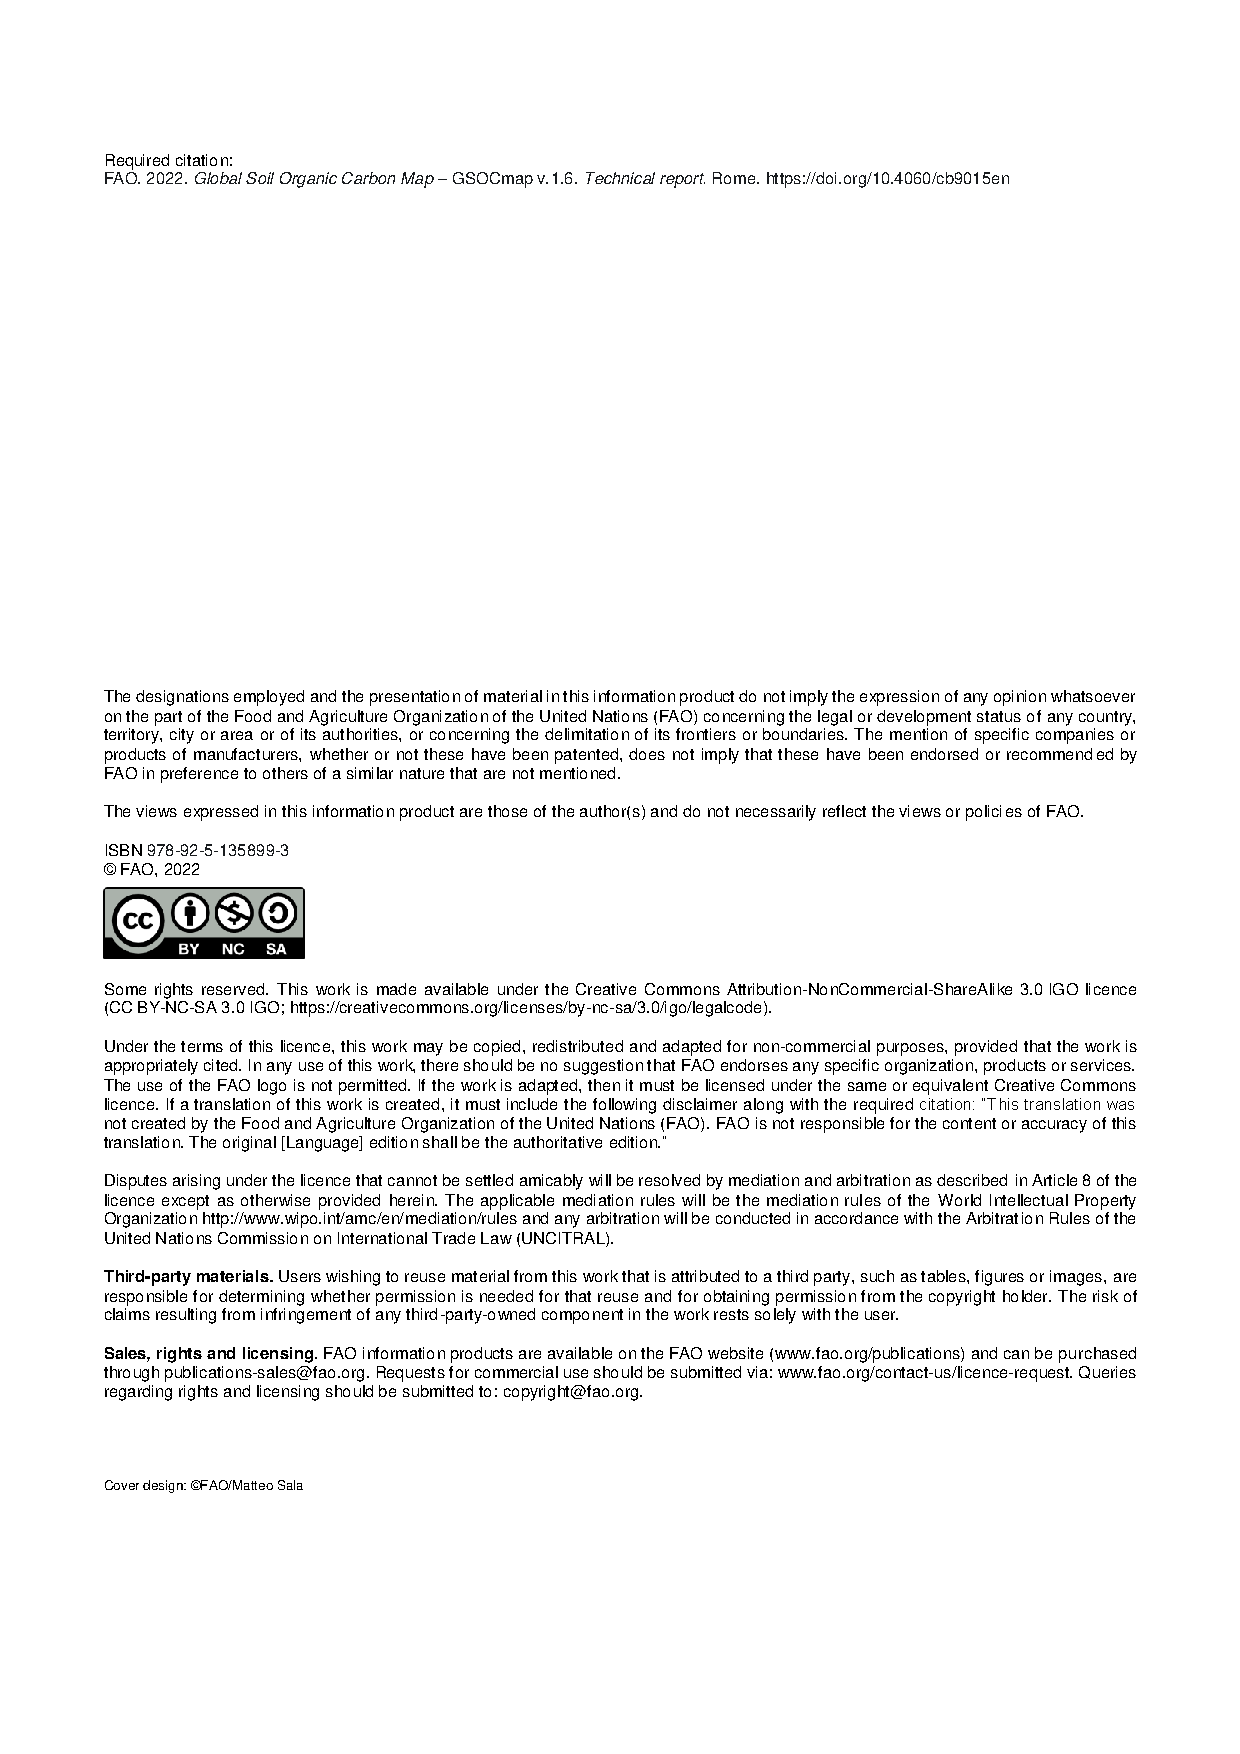
\includepdf{images/CB9015EN_Copyright Disclaimer_v2.pdf}


\hypertarget{licence}{%
\chapter*{Licence}\label{licence}}
\addcontentsline{toc}{chapter}{Licence}

Placeholder

\hypertarget{presentation}{%
\chapter{Presentation}\label{presentation}}

Placeholder

\hypertarget{global-soil-partnership}{%
\section{Global Soil Partnership}\label{global-soil-partnership}}

\hypertarget{country-driven-approach-and-tasks}{%
\section{Country-driven approach and tasks}\label{country-driven-approach-and-tasks}}

\hypertarget{how-to-use-this-book}{%
\section{How to use this book}\label{how-to-use-this-book}}

\hypertarget{training-material}{%
\section{Training material}\label{training-material}}

\hypertarget{soil-nutrients}{%
\chapter{Soil Nutrients}\label{soil-nutrients}}

Placeholder

\hypertarget{soil-properties-governing-nutrient-availability}{%
\section{Soil properties governing nutrient availability}\label{soil-properties-governing-nutrient-availability}}

\hypertarget{setting-up-the-software-environment}{%
\chapter{Setting-up the software environment}\label{setting-up-the-software-environment}}

Placeholder

\hypertarget{use-of-r-rstudio-and-r-packages}{%
\section{Use of R, RStudio and R Packages}\label{use-of-r-rstudio-and-r-packages}}

\hypertarget{obtaining-and-installing-r}{%
\subsection{Obtaining and installing R}\label{obtaining-and-installing-r}}

\hypertarget{obtaining-and-installing-rstudio}{%
\subsection{Obtaining and installing RStudio}\label{obtaining-and-installing-rstudio}}

\hypertarget{getting-started-with-r}{%
\subsection{Getting started with R}\label{getting-started-with-r}}

\hypertarget{r-packages}{%
\section{R packages}\label{r-packages}}

\hypertarget{gee---google-earth-engine}{%
\section{GEE - google earth engine}\label{gee---google-earth-engine}}

\hypertarget{rgee---extension-to-use-google-earth-engine-in-r}{%
\section{rgee - Extension to use google earth engine in R}\label{rgee---extension-to-use-google-earth-engine-in-r}}

\hypertarget{digital-soil-mapping}{%
\chapter{Digital Soil Mapping}\label{digital-soil-mapping}}

Placeholder

\hypertarget{principles}{%
\section{Principles}\label{principles}}

\hypertarget{environmental-covariates}{%
\section{Environmental covariates}\label{environmental-covariates}}

\hypertarget{machine-learning-techniques}{%
\section{Machine learning techniques}\label{machine-learning-techniques}}

\hypertarget{mapping-of-soil-nutrients-and-associated-soil-attributes}{%
\section{Mapping of soil nutrients and associated soil attributes}\label{mapping-of-soil-nutrients-and-associated-soil-attributes}}

\hypertarget{arranging-soil-data-in-r}{%
\chapter{\texorpdfstring{Arranging soil data in \textbf{R}}{Arranging soil data in R}}\label{arranging-soil-data-in-r}}

Placeholder

\hypertarget{study-area-and-training-material}{%
\section{Study area and training material}\label{study-area-and-training-material}}

\hypertarget{georeferenced-topsoil-data}{%
\subsection{Georeferenced topsoil data}\label{georeferenced-topsoil-data}}

\hypertarget{soil-profile-data}{%
\subsection{Soil profile data}\label{soil-profile-data}}

\hypertarget{preproc}{%
\section{Format requirements of soil data}\label{preproc}}

\hypertarget{pre-processing-steps}{%
\section{Pre-processing steps}\label{pre-processing-steps}}

\hypertarget{set-the-scene-set-working-directory-packages-load-data}{%
\subsection{Set the scene (set working directory, packages, load data)}\label{set-the-scene-set-working-directory-packages-load-data}}

\hypertarget{basic-data-handling-operations}{%
\subsection{Basic data handling operations}\label{basic-data-handling-operations}}

\hypertarget{step-1-soil-data-preparation}{%
\chapter{Step 1: soil data preparation}\label{step-1-soil-data-preparation}}

Placeholder

\hypertarget{load-national-data}{%
\section{Load national data}\label{load-national-data}}

\hypertarget{data-quality-check}{%
\section{Data quality check}\label{data-quality-check}}

\hypertarget{calculation-of-pedo-transfer-functions}{%
\section{Calculation of pedo-transfer functions}\label{calculation-of-pedo-transfer-functions}}

\hypertarget{check-for-outliers}{%
\section{Check for outliers}\label{check-for-outliers}}

\hypertarget{harmonise-soil-layer-depths}{%
\section{Harmonise soil layer depths}\label{harmonise-soil-layer-depths}}

\hypertarget{harmonise-units}{%
\section{Harmonise units}\label{harmonise-units}}

\hypertarget{save-the-results}{%
\section{Save the results}\label{save-the-results}}

\hypertarget{step-2-download-environmental-covariates}{%
\chapter{Step 2: download environmental covariates}\label{step-2-download-environmental-covariates}}

Placeholder

\hypertarget{environmental-covariates-1}{%
\section{Environmental covariates}\label{environmental-covariates-1}}

\hypertarget{download-covariates-with-rgee}{%
\section{Download covariates with rgee}\label{download-covariates-with-rgee}}

\hypertarget{obtaining-the-cropland-mask}{%
\section{Obtaining the cropland mask}\label{obtaining-the-cropland-mask}}

\hypertarget{step-3-mapping-continuous-soil-properties}{%
\chapter{Step 3: Mapping continuous soil properties}\label{step-3-mapping-continuous-soil-properties}}

Placeholder

\hypertarget{getting-prepared-to-map}{%
\section{Getting prepared to map}\label{getting-prepared-to-map}}

\hypertarget{covariate-selection-and-repeated-k-fold-cross-validation}{%
\section{Covariate selection and repeated k-fold cross-validation}\label{covariate-selection-and-repeated-k-fold-cross-validation}}

\hypertarget{model-calibration}{%
\section{Model calibration}\label{model-calibration}}

\hypertarget{uncertainty-assessment}{%
\section{Uncertainty assessment}\label{uncertainty-assessment}}

\hypertarget{predicting-soil-attributes}{%
\section{Predicting soil attributes}\label{predicting-soil-attributes}}

\hypertarget{reporting-results}{%
\chapter{Reporting results}\label{reporting-results}}

Placeholder

\hypertarget{data-submission-form}{%
\section{Data submission form}\label{data-submission-form}}

\hypertarget{way-forward}{%
\chapter{Way forward}\label{way-forward}}

This technical manual provided step-by-step guidance on how to generate nutrient maps by means of quantile regression forest models within a digital soil mapping framework. The array of maps produced belongs to the first implementation phase of the GSNmap initiative and provides urgently needed data on nutrient stocks and soil properties that govern nutrient availability. Policymakers will be able to use this data to derive conclusions on where to concentrate efforts to improve soil and land management to strengthen agrifood systems.
The second phase of the GSNmap will make use of the first phase data products to derive nutrient budget maps. Therefore, additional datasets will be used for calculating input and output terms of nutrient stocks. The methodology is currently under development by the GSNmap working group. The technical documentation towards implementing the second phase will be made available in mid 2023.

\hypertarget{frequent-asked-questions-and-troubleshooting-answers}{%
\section{Frequent asked questions and Troubleshooting answers}\label{frequent-asked-questions-and-troubleshooting-answers}}

To be developed soon\ldots{}

\hypertarget{issues-in-the-gsnmap-technical-manual}{%
\section{Issues in the GSNmap Technical Manual}\label{issues-in-the-gsnmap-technical-manual}}

Please, report any issue in the GSNmap Technical Manual in its issues GitHub page \url{https://github.com/FAO-GSP/GSNmap-TM/issues}.

\hypertarget{get-help}{%
\section{Get help}\label{get-help}}

\begin{itemize}
\tightlist
\item
  Check the issues GitHub page \url{https://github.com/FAO-GSP/GSNmap-TM/issues}
\item
  Issues with R packages: search for solutions in \url{https://stackoverflow.com/}
\item
  \texttt{caret} package \url{https://topepo.github.io/caret/}
\item
  \texttt{terra} package \url{https://rspatial.org/terra/pkg/1-introduction.html}
\item
  \texttt{tidyverse} package \url{https://r4ds.had.co.nz/}
\item
  \texttt{sf} package \url{https://r-spatial.github.io/sf/}
\end{itemize}

If these links do not help you, contact us including the following text:

\emph{I am {[}FULL NAME{]}, responsible for producing the GSNmap of {[}COUNTRY{]}.}

\href{mailto:marcos.angelini@fao.org}{\nolinkurl{marcos.angelini@fao.org}}

\hypertarget{annex-i-compendium-of-r-scripts}{%
\chapter*{Annex I: Compendium of R scripts}\label{annex-i-compendium-of-r-scripts}}
\addcontentsline{toc}{chapter}{Annex I: Compendium of R scripts}

Placeholder

\hypertarget{script-0-installation-of-rgee}{%
\section*{Script 0: Installation of rgee}\label{script-0-installation-of-rgee}}
\addcontentsline{toc}{section}{Script 0: Installation of rgee}

\hypertarget{script-1-data-preparation}{%
\section*{Script 1: Data preparation}\label{script-1-data-preparation}}
\addcontentsline{toc}{section}{Script 1: Data preparation}

\hypertarget{script-2-download-environmental-covariates}{%
\section*{Script 2: Download environmental covariates}\label{script-2-download-environmental-covariates}}
\addcontentsline{toc}{section}{Script 2: Download environmental covariates}

\hypertarget{script-3-modelling-validation-and-prediction-using-soil-data-with-coordinates}{%
\section*{Script 3: Modelling, validation and prediction using soil data with coordinates}\label{script-3-modelling-validation-and-prediction-using-soil-data-with-coordinates}}
\addcontentsline{toc}{section}{Script 3: Modelling, validation and prediction using soil data with coordinates}

\hypertarget{annex-iii-mapping-without-point-coordinates}{%
\chapter*{Annex III: Mapping without point coordinates}\label{annex-iii-mapping-without-point-coordinates}}
\addcontentsline{toc}{chapter}{Annex III: Mapping without point coordinates}

Placeholder

\hypertarget{annex-iv-quality-assurance-and-quality-control}{%
\chapter*{Annex IV: Quality assurance and quality control}\label{annex-iv-quality-assurance-and-quality-control}}
\addcontentsline{toc}{chapter}{Annex IV: Quality assurance and quality control}

The following protocol was devised to provide National Experts with a step-by-step guideline to perform a Quality Assurance (QA) and Quality Control (QC) of the 10 GSNmap first phase products.

The following protocol does not provide any guidance in terms of uncertainty estimation and validation. For more details and information on the estimation of uncertainties and potential map validation strategies please refer to Chapter 8.4.

Quality assurance and quality control consist of activities to ensure the quality of a particular result. Quality control is a reactive process that focuses on identifying defects and errors while quality assurance is a proactive approach aimed at preventing defects and errors. In the context of digital soil mapping, both processes are often interlinked. A QA is interlinked with a QC when it identifies defects and the QA remodels the process to eliminate the defects and prevent them from recurring (Chapman, 2005)(Figure@ref(fig:qa\_qc)).

\begin{figure}
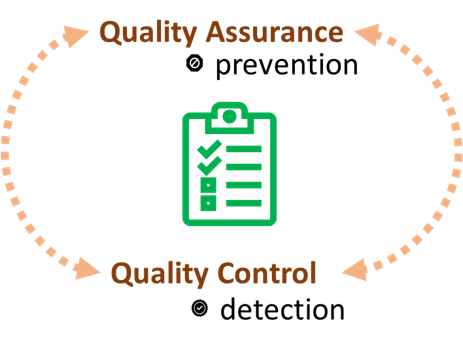
\includegraphics[width=6.43in]{images/QA_QC} \caption{Quality assurance and quality control.}(\#fig:qa_qc)
\end{figure}

Each step in the following protocol should be considered in order to detect and eliminate errors, address data inaccuracies and assess the output completeness.

\hypertarget{step-1-completeness-of-layers}{%
\section*{Step 1: Completeness of layers}\label{step-1-completeness-of-layers}}
\addcontentsline{toc}{section}{Step 1: Completeness of layers}

The following Table \ref(tab:products) gives an overview of all the GSNmap products in alphabetical order. Each product should include the ISO 3166-1 alpha-3 country code as uppercase letters in its name. For instance, in the case of Turkiye, ISO\_GSNmap\_Ntot\_Map030 should be changed to TUR\_GSNmap\_Ntot\_Map030.

All 10 soil property and soil nutrient maps with their corresponding 10 uncertainty layers must be georeferenced TIF (.tif) files.

\label{tab:products}\label{tab:products}Data product overview.

Product

Filename

Major nutrients (3 files)

Total Nitrogen map

ISO\_GSNmap\_Ntot\_Map030.tiff

Available Phosphorus map

ISO\_GSNmap\_Pav\_Map030.tiff

Total Potassium map

ISO\_GSNmap\_Ktot\_Map030.tiff

Associated soil properties (7 files)

Cation exchange capacity map

ISO\_GSNmap\_CEC\_Map030.tiff

Soil pH map

ISO\_GSNmap\_pH\_Map030.tiff

Soil clay map

ISO\_GSNmap\_Clay\_Map030.tiff

Soil silt map

ISO\_GSNmap\_Silt\_Map030.tiff

Soil sand map

ISO\_GSNmap\_Sand\_Map030.tiff

Soil organic carbon map

ISO\_GSNmap\_SOC\_Map030.tiff

Soil bulk density map

ISO\_GSNmap\_BD\_Map030.tiff

Uncertainty maps (10 files)

Total Nitrogen uncertainty map

ISO\_GSNmap\_Ntot\_UncertaintyMap030.tiff

Available Phosphorus uncertainty map

ISO\_GSNmap\_Pav\_UncertaintyMap030.tiff

Total Potassium uncertainty map

ISO\_GSNmap\_Ktot\_UncertaintyMap030.tiff

Cation exchange capacity uncertainty map

ISO\_GSNmap\_CEC\_UncertaintyMap030.tiff

Soil pH uncertainty map

ISO\_GSNmap\_pH\_UncertaintyMap030.tiff

Soil clay uncertainty map

ISO\_GSNmap\_Clay\_UncertaintyMap030.tiff

Soil silt uncertainty map

ISO\_GSNmap\_Silt\_UncertaintyMap030.tiff

Soil sand uncertainty map

ISO\_GSNmap\_Sand\_UncertaintyMap030.tiff

Soil organic carbon uncertainty map

ISO\_GSNmap\_SOC\_UncertaintyMap030.tiff

Soil bulk density uncertainty map

ISO\_GSNmap\_BD\_UncertaintyMap030.tiff

\hypertarget{step-2-check-the-projection-and-resolution-of-all-data-products}{%
\section*{Step 2: Check the projection and resolution of all data products}\label{step-2-check-the-projection-and-resolution-of-all-data-products}}
\addcontentsline{toc}{section}{Step 2: Check the projection and resolution of all data products}

Open the products in QGIS or any other preferred GIS platform. Check that the projection of all products is EPSG:4326 - WGS 84 (Layer properties). Check that the spatial resolution (pixel size) (Layer properties) is equal to \textasciitilde0.002246 degrees ; 250 m x 250 m at the equator.

\hypertarget{step-3-check-the-extent}{%
\section*{Step 3: Check the extent}\label{step-3-check-the-extent}}
\addcontentsline{toc}{section}{Step 3: Check the extent}

Visualize the 20 products in QGIS or any preferred GIS platform. Load a land-use layer to visually assess that the simulations were done exclusively on croplands.

\hypertarget{step-4-check-the-units-ranges-and-outliers}{%
\section*{Step 4: Check the units, ranges, and outliers}\label{step-4-check-the-units-ranges-and-outliers}}
\addcontentsline{toc}{section}{Step 4: Check the units, ranges, and outliers}

In the following section possible value ranges for each product category (except available potassium) are presented. It is important to note that the provided ranges represent a gross approximation of the extremes within which the values should fall in. Results that fall outside these ranges need to be carefully evaluated based on local expertise and available literature.

The provided ranges can be compared in QGIS, R, or any preferred platform. Descriptive layer statistics can be viewed in QGIS under Layer Properties.

The following table (Table 10.2) presents ranges of possible values for 9 of the 10 mandatory GSNmap products. The ranges were calculated based on the distribution of the soil profile data within the World Soil Information Service (WoSIS), specifically the WoSIS snapshot 2019 (Batjes, N. H. \emph{et al.} 2020). It is important to note that the data was not filtered for croplands and that the ranges were extracted from soil profiles sampled globally from a wide array of land covers and land uses.

\label{tab:ranges}\label{tab:ranges}Possible soil property and soil nutrient values based on the distribution of the values within the World Soil Information Service (WoSIS), specifically the WoSIS snapshot 2019.

Soil property

Min

1st Quartile

Median

3st Quartile

Max

n

Unit

Total N

0.0

400.0

700.0

1500.0

84000.0

216362

ppm

P Bray I

0.0

1.6

5.0

16.0

150.0

40486

ppm

P Mehlich 3

0.0

1.6

6.1

22.0

149.4

7242

ppm

P Olsen

0.0

0.7

2.0

4.3

141.0

8434

ppm

CEC

0.1

7.5

14.0

23.0

140.0

295688

cmol(c)/kg

pH water

1.5

5.2

6.2

7.5

12.3

613322

\begin{itemize}
\item
  Clay

  0.0

  11.1

  21.9

  35.3

  100.0

  590368

  \%

  Silt

  0.0

  15.0

  30.0

  47.6

  100.0

  558233

  \%

  Sand

  0.0

  15.0

  36.0

  60.2

  100.0

  482334

  \%

  SOC

  0.0

  2.0

  5.1

  14.0

  99.4

  471301

  \%

  Bulk density

  0.0

  1.3

  1.4

  1.7

  2.6

  116756

  g/cm3
\end{itemize}

\hypertarget{references}{%
\chapter*{References}\label{references}}
\addcontentsline{toc}{chapter}{References}

%\printindex
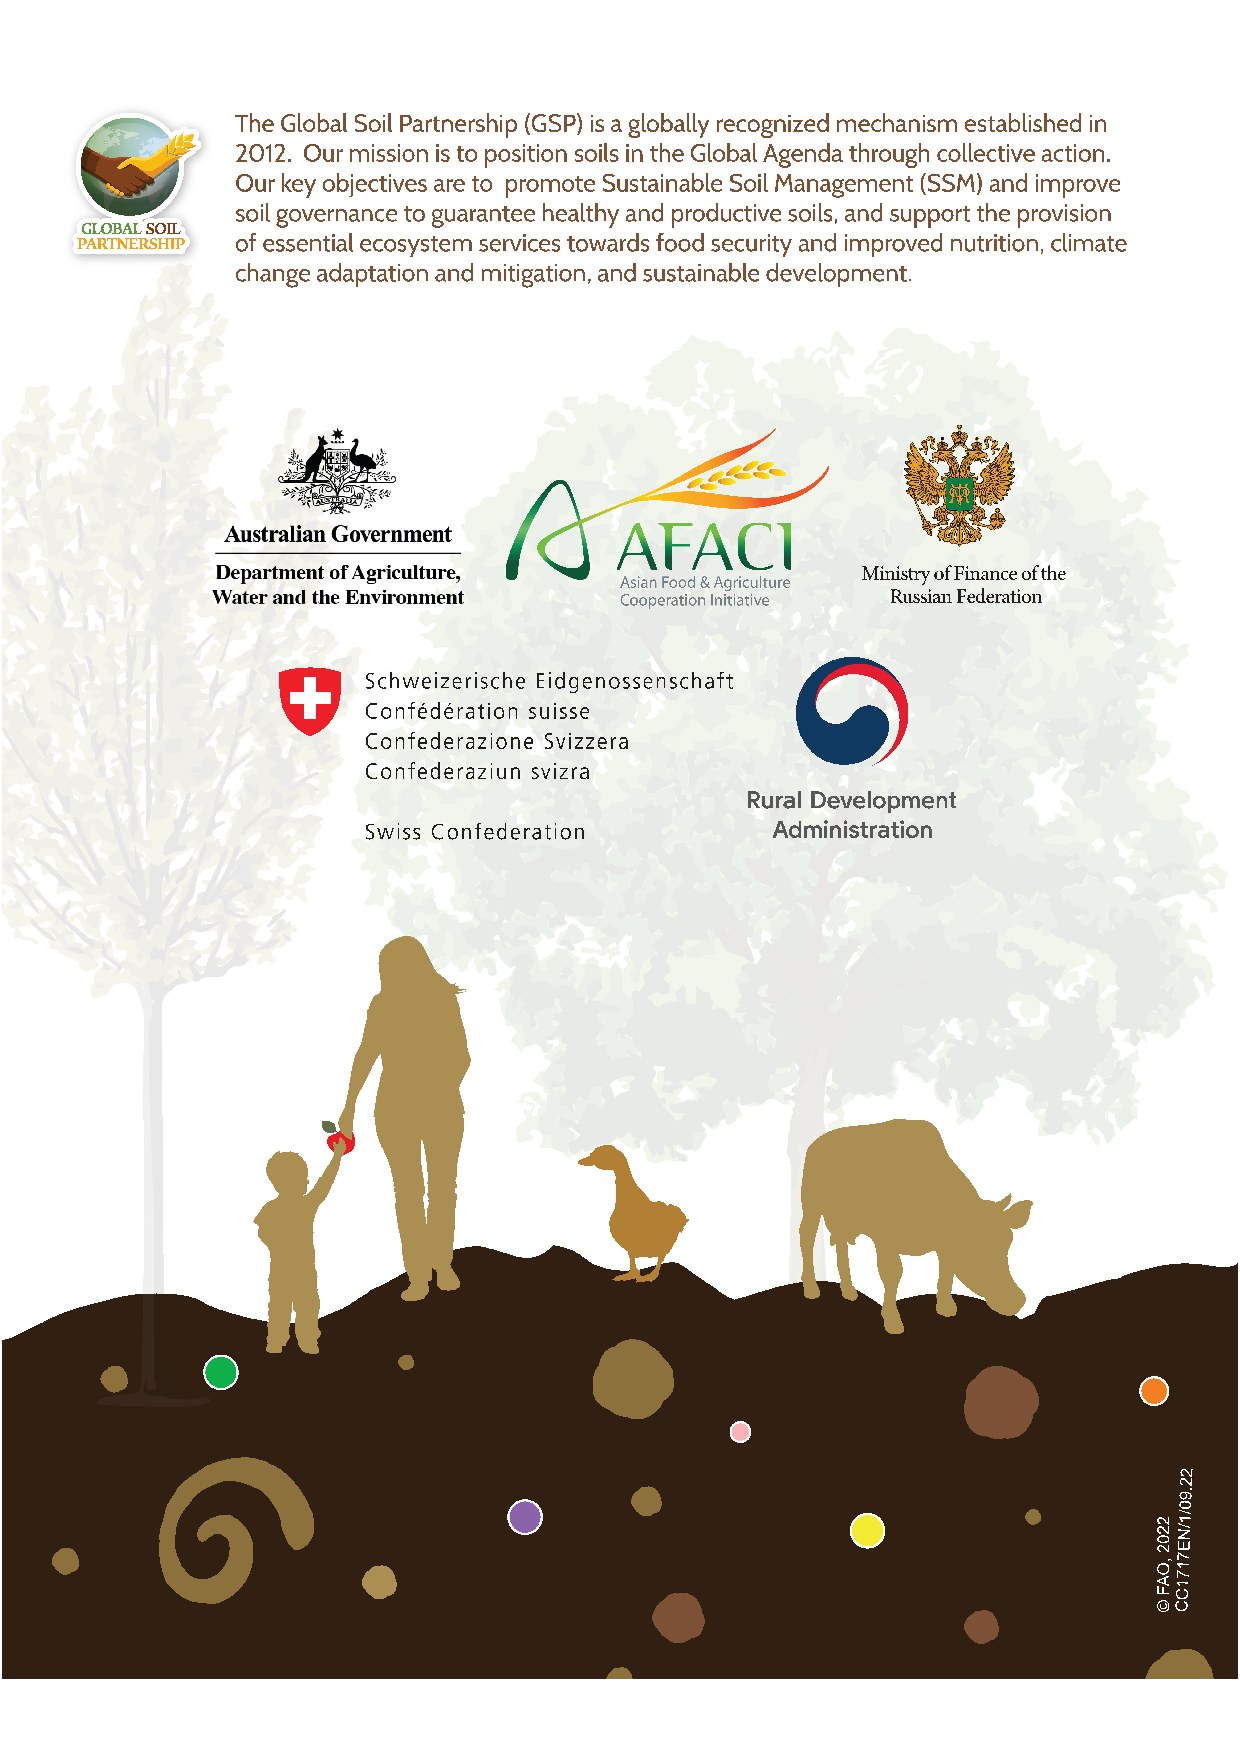
\includepdf{images/backcover.pdf}

\end{document}
